% Editable source for result.pdf, written by make_result_figure.py from run_github_39527549698/panel/result.json
\documentclass[tikz,border=6pt]{standalone}
\usepackage[T1]{fontenc}
\begin{document}
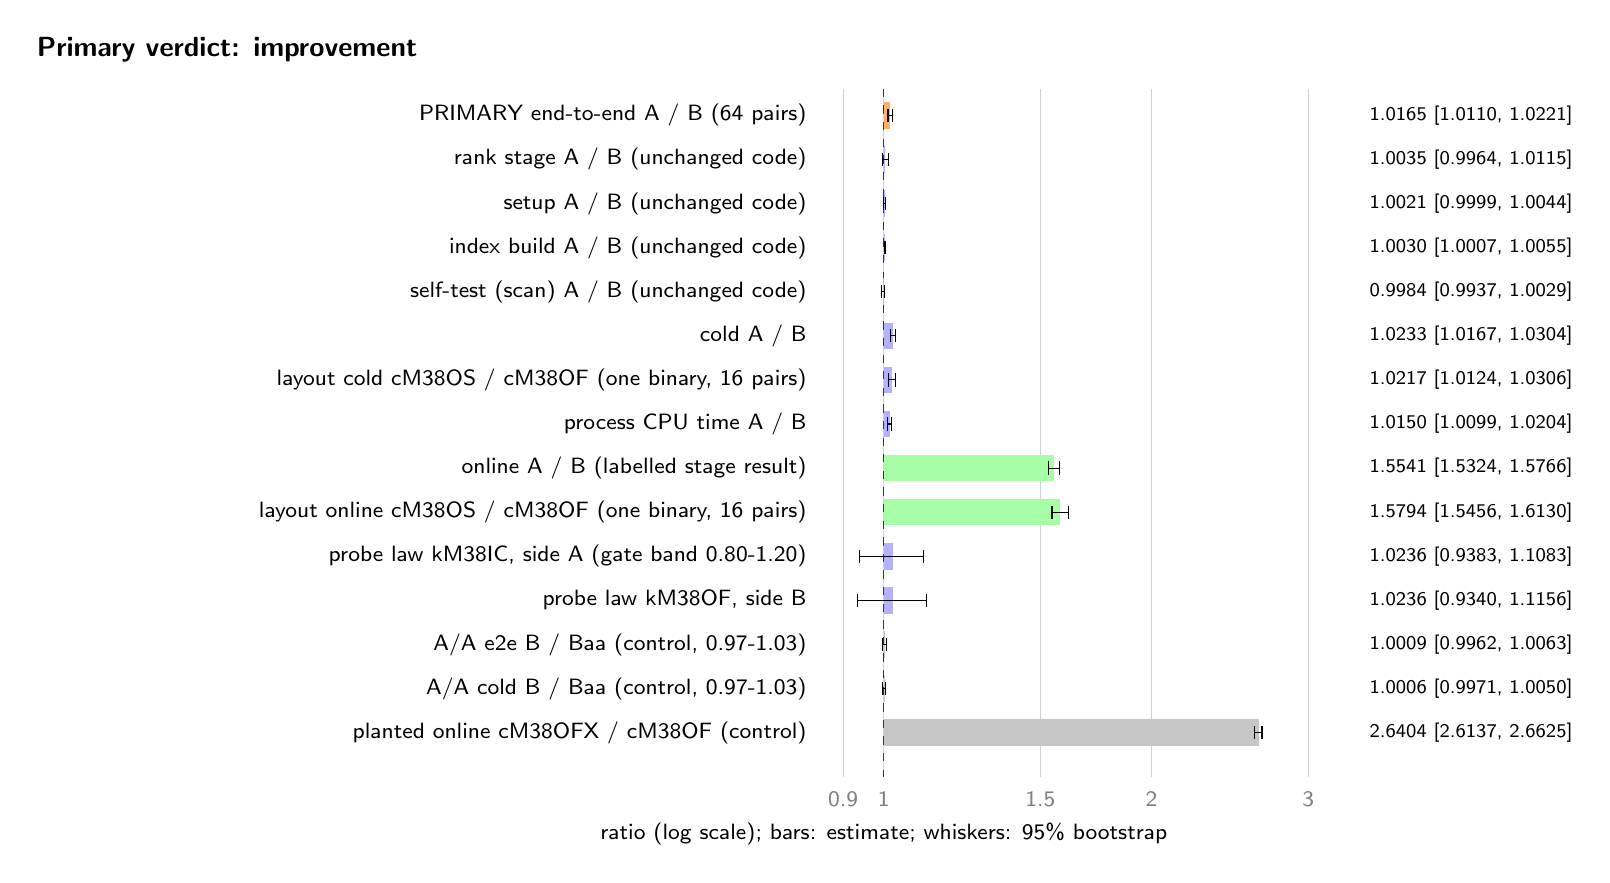
\begin{tikzpicture}[font=\sffamily\footnotesize,x=34mm,y=-5.6mm]
\draw[gray!35] (-0.1520,-0.6) -- (-0.1520,15); \node[gray] at (-0.1520,15.5) {0.9};
\draw[gray!35] (0.0000,-0.6) -- (0.0000,15); \node[gray] at (0.0000,15.5) {1};
\draw[gray!35] (0.5850,-0.6) -- (0.5850,15); \node[gray] at (0.5850,15.5) {1.5};
\draw[gray!35] (1.0000,-0.6) -- (1.0000,15); \node[gray] at (1.0000,15.5) {2};
\draw[gray!35] (1.5850,-0.6) -- (1.5850,15); \node[gray] at (1.5850,15.5) {3};
\draw[red!70!black,dashed] (0,-0.6) -- (0,15);
\node at (0,16.3) {ratio (log scale); bars: estimate; whiskers: 95\% bootstrap};
\node[anchor=west,font=\sffamily\bfseries] at (-3.2,-1.5) {Primary verdict: improvement};
\node[anchor=east] at (-0.2520,0) {PRIMARY end-to-end A / B (64 pairs)};
\fill[orange!60] (0,-0.300000) rectangle (0.0236,0.300000);
\draw (0.0158,0) -- (0.0316,0); \draw (0.0158,-0.150000) -- (0.0158,0.150000); \draw (0.0316,-0.150000) -- (0.0316,0.150000);
\node[anchor=west,font=\sffamily\scriptsize] at (1.7781,0) {1.0165 [1.0110, 1.0221]};
\node[anchor=east] at (-0.2520,1) {rank stage A / B (unchanged code)};
\fill[blue!30] (0,0.700000) rectangle (0.0050,1.300000);
\draw (-0.0052,1) -- (0.0165,1); \draw (-0.0052,0.850000) -- (-0.0052,1.150000); \draw (0.0165,0.850000) -- (0.0165,1.150000);
\node[anchor=west,font=\sffamily\scriptsize] at (1.7781,1) {1.0035 [0.9964, 1.0115]};
\node[anchor=east] at (-0.2520,2) {setup A / B (unchanged code)};
\fill[blue!30] (0,1.700000) rectangle (0.0031,2.300000);
\draw (-0.0001,2) -- (0.0064,2); \draw (-0.0001,1.850000) -- (-0.0001,2.150000); \draw (0.0064,1.850000) -- (0.0064,2.150000);
\node[anchor=west,font=\sffamily\scriptsize] at (1.7781,2) {1.0021 [0.9999, 1.0044]};
\node[anchor=east] at (-0.2520,3) {index build A / B (unchanged code)};
\fill[blue!30] (0,2.700000) rectangle (0.0044,3.300000);
\draw (0.0011,3) -- (0.0079,3); \draw (0.0011,2.850000) -- (0.0011,3.150000); \draw (0.0079,2.850000) -- (0.0079,3.150000);
\node[anchor=west,font=\sffamily\scriptsize] at (1.7781,3) {1.0030 [1.0007, 1.0055]};
\node[anchor=east] at (-0.2520,4) {self-test (scan) A / B (unchanged code)};
\fill[blue!30] (0,3.700000) rectangle (-0.0023,4.300000);
\draw (-0.0092,4) -- (0.0041,4); \draw (-0.0092,3.850000) -- (-0.0092,4.150000); \draw (0.0041,3.850000) -- (0.0041,4.150000);
\node[anchor=west,font=\sffamily\scriptsize] at (1.7781,4) {0.9984 [0.9937, 1.0029]};
\node[anchor=east] at (-0.2520,5) {cold A / B};
\fill[blue!30] (0,4.700000) rectangle (0.0332,5.300000);
\draw (0.0239,5) -- (0.0431,5); \draw (0.0239,4.850000) -- (0.0239,5.150000); \draw (0.0431,4.850000) -- (0.0431,5.150000);
\node[anchor=west,font=\sffamily\scriptsize] at (1.7781,5) {1.0233 [1.0167, 1.0304]};
\node[anchor=east] at (-0.2520,6) {layout cold cM38OS / cM38OF (one binary, 16 pairs)};
\fill[blue!30] (0,5.700000) rectangle (0.0310,6.300000);
\draw (0.0177,6) -- (0.0435,6); \draw (0.0177,5.850000) -- (0.0177,6.150000); \draw (0.0435,5.850000) -- (0.0435,6.150000);
\node[anchor=west,font=\sffamily\scriptsize] at (1.7781,6) {1.0217 [1.0124, 1.0306]};
\node[anchor=east] at (-0.2520,7) {process CPU time A / B};
\fill[blue!30] (0,6.700000) rectangle (0.0215,7.300000);
\draw (0.0142,7) -- (0.0291,7); \draw (0.0142,6.850000) -- (0.0142,7.150000); \draw (0.0291,6.850000) -- (0.0291,7.150000);
\node[anchor=west,font=\sffamily\scriptsize] at (1.7781,7) {1.0150 [1.0099, 1.0204]};
\node[anchor=east] at (-0.2520,8) {online A / B (labelled stage result)};
\fill[green!35] (0,7.700000) rectangle (0.6361,8.300000);
\draw (0.6158,8) -- (0.6568,8); \draw (0.6158,7.850000) -- (0.6158,8.150000); \draw (0.6568,7.850000) -- (0.6568,8.150000);
\node[anchor=west,font=\sffamily\scriptsize] at (1.7781,8) {1.5541 [1.5324, 1.5766]};
\node[anchor=east] at (-0.2520,9) {layout online cM38OS / cM38OF (one binary, 16 pairs)};
\fill[green!35] (0,8.700000) rectangle (0.6594,9.300000);
\draw (0.6282,9) -- (0.6898,9); \draw (0.6282,8.850000) -- (0.6282,9.150000); \draw (0.6898,8.850000) -- (0.6898,9.150000);
\node[anchor=west,font=\sffamily\scriptsize] at (1.7781,9) {1.5794 [1.5456, 1.6130]};
\node[anchor=east] at (-0.2520,10) {probe law kM38IC, side A (gate band 0.80-1.20)};
\fill[blue!30] (0,9.700000) rectangle (0.0337,10.300000);
\draw (-0.0918,10) -- (0.1484,10); \draw (-0.0918,9.850000) -- (-0.0918,10.150000); \draw (0.1484,9.850000) -- (0.1484,10.150000);
\node[anchor=west,font=\sffamily\scriptsize] at (1.7781,10) {1.0236 [0.9383, 1.1083]};
\node[anchor=east] at (-0.2520,11) {probe law kM38OF, side B};
\fill[blue!30] (0,10.700000) rectangle (0.0337,11.300000);
\draw (-0.0985,11) -- (0.1578,11); \draw (-0.0985,10.850000) -- (-0.0985,11.150000); \draw (0.1578,10.850000) -- (0.1578,11.150000);
\node[anchor=west,font=\sffamily\scriptsize] at (1.7781,11) {1.0236 [0.9340, 1.1156]};
\node[anchor=east] at (-0.2520,12) {A/A e2e B / Baa (control, 0.97-1.03)};
\fill[gray!45] (0,11.700000) rectangle (0.0013,12.300000);
\draw (-0.0055,12) -- (0.0091,12); \draw (-0.0055,11.850000) -- (-0.0055,12.150000); \draw (0.0091,11.850000) -- (0.0091,12.150000);
\node[anchor=west,font=\sffamily\scriptsize] at (1.7781,12) {1.0009 [0.9962, 1.0063]};
\node[anchor=east] at (-0.2520,13) {A/A cold B / Baa (control, 0.97-1.03)};
\fill[gray!45] (0,12.700000) rectangle (0.0008,13.300000);
\draw (-0.0042,13) -- (0.0072,13); \draw (-0.0042,12.850000) -- (-0.0042,13.150000); \draw (0.0072,12.850000) -- (0.0072,13.150000);
\node[anchor=west,font=\sffamily\scriptsize] at (1.7781,13) {1.0006 [0.9971, 1.0050]};
\node[anchor=east] at (-0.2520,14) {planted online cM38OFX / cM38OF (control)};
\fill[gray!45] (0,13.700000) rectangle (1.4007,14.300000);
\draw (1.3861,14) -- (1.4128,14); \draw (1.3861,13.850000) -- (1.3861,14.150000); \draw (1.4128,13.850000) -- (1.4128,14.150000);
\node[anchor=west,font=\sffamily\scriptsize] at (1.7781,14) {2.6404 [2.6137, 2.6625]};
\end{tikzpicture}
\end{document}
